\chapter{ Аналитический раздел}
\label{cha:analysis}

\section{Некоторые теоретические сведения}

Для начала нужно ввести собственно понятие матрицы.

\textit{Матрица} -- объект, записываемый в виде прямоугольной таблицы элементов,
которая представляет собой совокупность строк и столбцов, на пересечении которых находятся её элементы (формула \ref{eq:ref1}).

\begin{equation}
	A = \left(
	\begin{array}{cccc}
			a_{11} & a_{12} & \ldots & a_{1n} \\
			a_{21} & a_{22} & \ldots & a_{2n} \\
			\vdots & \vdots & \ddots & \vdots \\
			a_{n1} & a_{n2} & \ldots & a_{nn}
		\end{array}
	\right)
	\label{eq:ref1}
\end{equation}

\textit{Произведение матриц} AB состоит из всех возможных комбинаций скалярных произведений 
вектор-строк матрицы A и вектор-столбцов матрицы B (рис. \ref{fg:ref2}).

\begin{figure}[ht!]
	\centering{
		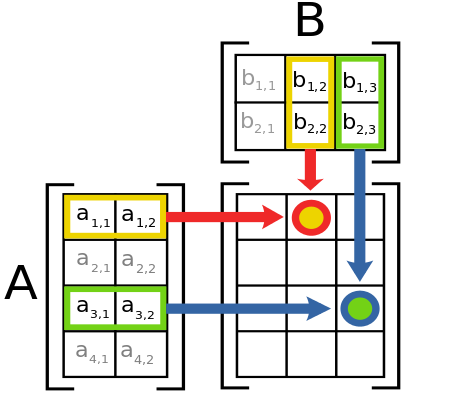
\includegraphics[width=0.5\textwidth]{img/matrix_mult.png}
		\caption{Произведение матриц}
		\label{fg:ref2}}
\end{figure}

Операция умножения двух матриц выполнима только в том случае, если число столбцов в первой матрице равно числу строк во второй.

\section{Стандартный алгоритм умножения матриц}

Допустим имеется матрицы A (формула \ref{eq:ref1}) и B (формула \ref{eq:ref2})

\begin{equation}
	B = \left(
	\begin{array}{cccc}
			b_{11} & b_{12} & \ldots & b_{1n} \\
			b_{21} & b_{22} & \ldots & b_{2n} \\
			\vdots & \vdots & \ddots & \vdots \\
			b_{n1} & b_{n2} & \ldots & b_{nn}
		\end{array}
	\right)
	\label{eq:ref2}
\end{equation}

Матрица C = AB будет размерностью $l \times n$, 
где матрица A размерностью $l \times m$, а матрица B $m \times n$
Тогда каждый элемент матрицы C выражается формулой (\ref{eq:ref3})

\begin{equation}
	\begin{array}{cc}
		c_{ij} = \sum\limits_{r=1}^m a_{ir}b_{ri} & (i=1,2,\dots l; j=1,2,\dots n)
	\end{array}
	\label{eq:ref3}
\end{equation}

\section{Умножение матриц по Винограду}

Каждый элемент в матрице C, которая является результатом умножения двух матриц,
представляет собой скалярное произведение соответствующих строки и столбца исходных матриц. 
В алгоритме умножение матриц по Винограду предложено сделать предварительную обработку,
позволяющую часть работы выполнить заранее.

Рассмотрим два вектора V (формула \ref{eq:ref4}) и W (формула \ref{eq:ref5}).

\begin{equation}
	V = (v_1, v_2, v_3, v_4)
	\label{eq:ref4}
\end{equation}

\begin{equation}
	W = (w_1, w_2, w_3, w_4)
	\label{eq:ref5}
\end{equation}

Их скалярное произведение равно  \ref{eq:ref6}.

\begin{equation}
	V * W = v_1w_1 + v_2w_2 + v_3w_3 + v_4w_4
	\label{eq:ref6}
\end{equation}

Равенство \ref{eq:ref6} можно записать в виде \ref{eq:ref7}.

\begin{equation}
	\begin{array}{l}
		V * W = (v_1 + w_2)(v_2 + w_1) + (v_3 + w_4)(v_4 + w_3) - \\
		\quad \quad \quad v_1v_2 - v_3v_4 - w_1w_2 - w_3w_4
	\end{array}
	\label{eq:ref7}
\end{equation}

Выражение в правой части равенства \ref{eq:ref7} допускает предварительную обработку:
его части можно вычислить заранее и запомнить для каждой строки первой матрицы и для каждого столбца второй. На практике это означает,
что над предварительно обработанными элементами нам придется выполнять лишь первые два умножения и последующие пять сложений, а
также дополнительно два сложения.

\section{Вывод}

Были рассмотрены основополагающие материалами, которые в дальнейшем потребуются при реализации алгоритмов умножения матриц.  



